\begin{figure}[tb]
  \centering
  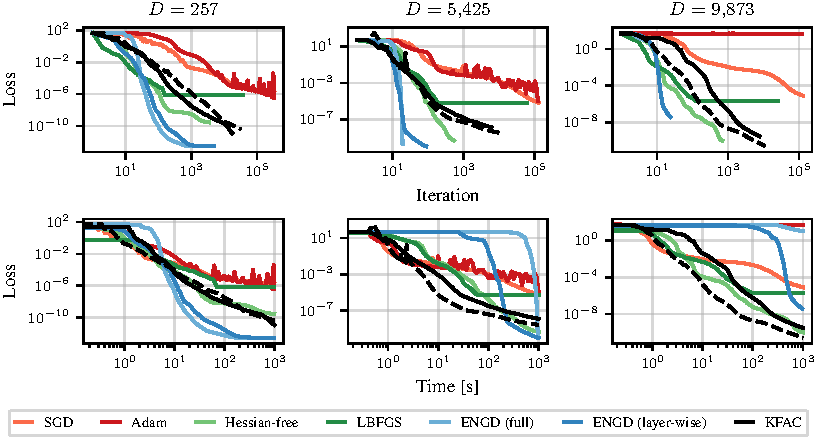
\includegraphics{../kfac_pinns_exp/exp17_groupplot_poisson2d/loss.pdf}
  \caption{Scaling behaviour of different optimizers for learning the solution of a 2d-Poisson equation w.r.t.
    neural network size under a given time budget of $10^3\,\text{s}$ on an RTX 6000 GPU.}
  \label{fig:pedagogical-example}
\end{figure}

\subsection{Setup}

Small-scale example (2D Poisson?)
\begin{itemize}
    \item Tested optimizers: Adam, GD with LS?, Newton's method / (L-)BFGS, Full ENGD, (Block)-Diagonal approximation for ENGD?, KFAG, other KFACs: for the l2-GN, empirical Fisher, Quantum KFAC
    \item damping: try both constant and adaptive damping
    \item try without line search with learning rate schedule
\end{itemize}

\begin{itemize}
    \item use weights and biases for large scale experiments
    \item next steps: modular code
\end{itemize}

\subsection{The Poisson equation}

\subsection{asdf}

We want to show the following things:
\begin{itemize}
\item We can safely discard the Gramian's off-diagonal blocks without harming
  training performance. This reduces the Gramian's size, but still imposes
  strong constraints on scalability.

\item Our proposed Kronecker approximation works roughly as well as the
  full/block diagonal Gramian, while being much cheaper to compute, store, and
  invert.

\item Thanks to the Kronecker approximation of the Gramian, we can scale to larger neural networks where the other methods either do not work (storing the Gramian is prohibitively expensive) or become quite slow (matrix-free linear system solve via Gramian-vector products).
\end{itemize}

Todos:
\begin{itemize}
\item concrete example ground truth: 2d Poisson on unit square with sine target
\end{itemize}

Ideas:
\begin{itemize}
\item try out different approximations
  \begin{itemize}
  \item Ground truth
  \item Block diagonal exact
  \item Diagonal
  \item Block diagonal with different approximations
  \end{itemize}
\end{itemize}

%%% Local Variables:
%%% mode: latex
%%% TeX-master: "../main"
%%% End:
